%--------------------------------------------------------
\section{Deployment} \label{sec:deployment}
%--------------------------------------------------------



%--------------------------------------------------------
\subsection{coexist.ini file}  \label{sec:ini}


% use relative file paths

\begin{itemize}
\item \bt{name} The name of the application. It will be seen in the main window of the Android application, title of Web pages etc.
\item \bt{image} An image icon for the application. On Android, this will be the icon that users click to launch the application.
\item \bt{notification} An image icon for the application's notifications. This can optionally be the same as the \bt{image} parameter, but most Android applications have a grey scale version of \bt{image} here instead.
\item \bt{package} The unique java style domain for your application. If a particular instance is going to be an inventory application for a company with the domain \bt{domain.com} then this field might be \bt{com.domain.inventory}. This field is important because Android requires all applications to have a unique package name. 
\item \bt{api} The URL of the Coexist server API. If this is the first time Coexist is being configured then the server API would not have been deployed yet, but the location is still required. This field could be \bt{http://domain.com/api/}; this is the URL that the clients will send their requests to. 
\item \bt{version} This is the current version of the application (i.e. 1). This will ultimately reside in a directory of the server API (that gets created using this file) \bt{conf/conf.ini}. If it is ever incremented then it will reject all client requests that are using different versions with a 409 error code and cause them to resync and upgrade. More on this in the server section ??.
\item \bt{user} The user name of the database for the server API's use.
\item \bt{pass} The password of the database for the server API's use.
\item \bt{db} The name of the database for the server API's use.
\item \bt{host} The hostname of the database for the server API's use.
\item \bt{dbms} The database type (i.e. mysql, postgresql) for use in the server API's PHP PDO calls. It should support any database type that the PDO library does.
\item \bt{ui} The location of the ui dir that should be included in the server API. This is explained further in the UI Dir section ??.
\item \bt{sql} The location of the sql dir that should be included in the server API. This is explained further in the SQL Dir section ??.
\item \bt{android} An on/off value can be used to enable or disable the Android build.
\item \bt{Web} An on/off value can be used to enable or disable the server API build.
\item \bt{scp\_to} An experimental key that can be used to better automate the build process. A possible value might be \bt{user@domain.com:/srv/domain.com/}. This would cause the resulting apk and tgz packages to be copied to the target server using scp. The public facing content in the tgz package is in a folder named htdocs, so the sample \texttt{scp\_to} value would be especially wise if the document root was \texttt{/srv/domain.com/htdocs} because a simple un-tar would be all that was required. 
\item \bt{scp\_port} Just in case the ssh server is running on a non standard port.
\end{itemize}





%--------------------------------------------------------
\subsection{Create the database.}  \label{sec:}

ShoppingList is a simple application, consisting of one table called
\texttt{Items}. Create the database and a user on the server, and execute the
SQL to create the desired table and meta data trigger. Its not hard to manually
create the triggers when there are few tables, but it can be tedious as more
tables are added. In \texttt{Web/bin}, there is a script called
\texttt{mktriggers} that will parse SQL files and send triggers to stdout. A
version of this file should also be saved in \texttt{Web/lib/SQL/SQLite/1}.
Saving it in this location means that it will be given to clients that use
Sqlite for version \texttt{1} of the application.


\begin{figure}[h!]
\begin{lstlisting}[language=sql]
REATE TABLE Items(
  item VARCHAR(100),
  mod_ts DATETIME, --metacolumn
  deleted INTEGER, --metacolumn
  CONSTRAINT item_pk PRIMARY KEY (item)
);

CREATE TRIGGER Items_trigger 
  BEFORE UPDATE ON Items 
  FOR EACH ROW SET NEW.mod_ts=NOW();
\end{lstlisting}
\caption{ShoppingList SQL file.}
\label{fig:shoppinglist_SQL}
\end{figure}




%--------------------------------------------------------
\subsection{Create the JSON meta model.}  \label{sec:}

A simple database requires an equally simple JSON meta model. The following
model will create a single \textit{Items} form on the client, consisting of the
\texttt{text field} \textit{Item}. This file should be saved in
\texttt{Web/lib/ui/1/}, for the same reasons as the previous SQL file.

\begin{figure}[h!]
\begin{lstlisting}[language=json]
{
  "forms" : [
  { 
    "label":"Items",
    "table":"Items",
    "fields": [
    {"label":"Item", "type":"text","column":"item"}
    ]
  }
  ]
}
\end{lstlisting}
\caption{ShoppingList JSON meta model.}
\label{fig:shoppinglist_json}
\end{figure}













%--------------------------------------------------------
\subsection{Start the Android application and let it sync.}  \label{sec:}

Once the application is installed and opened, the screen will be blank and spinning. 


\begin{figure}[h!]
\centering
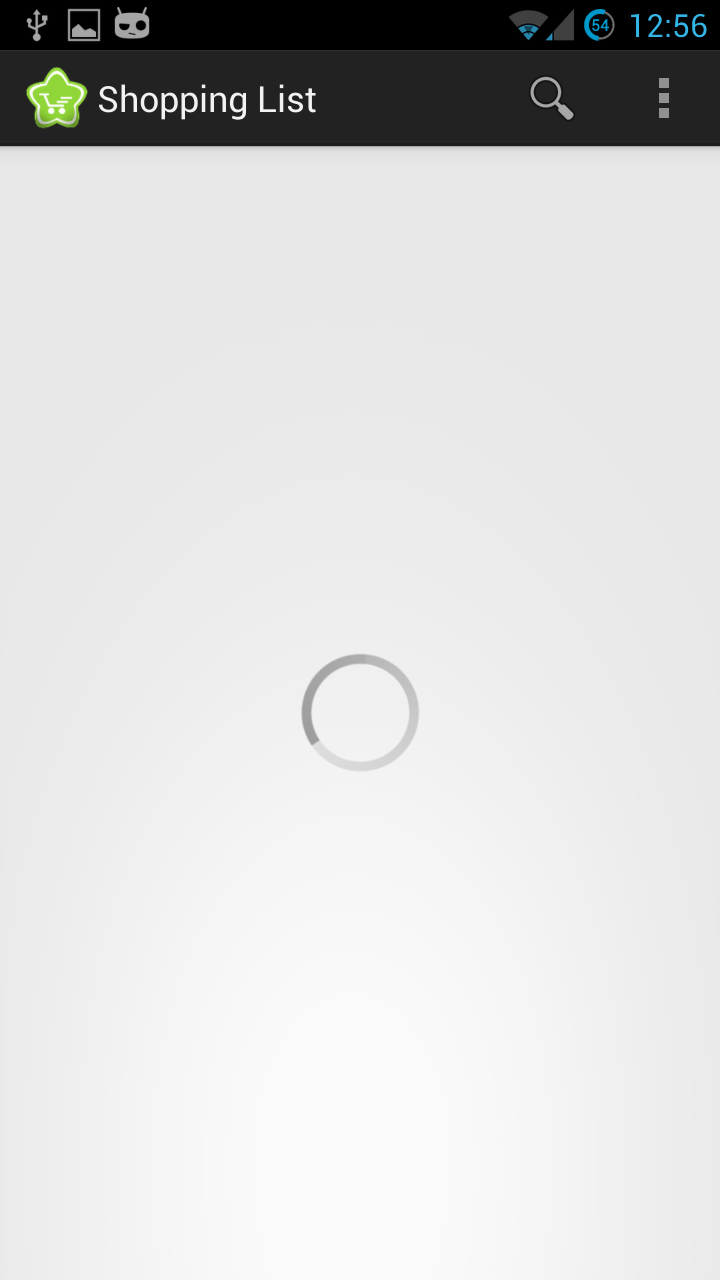
\includegraphics[width=0.25\textwidth]{images/new.png}
\caption{ShoppingList on first launch.}
\label{fig:first_launch}
\end{figure}

In the overflow menu there is an option called \texttt{Sync Now} that will trigger a sync.


\begin{figure}[h!]
\centering
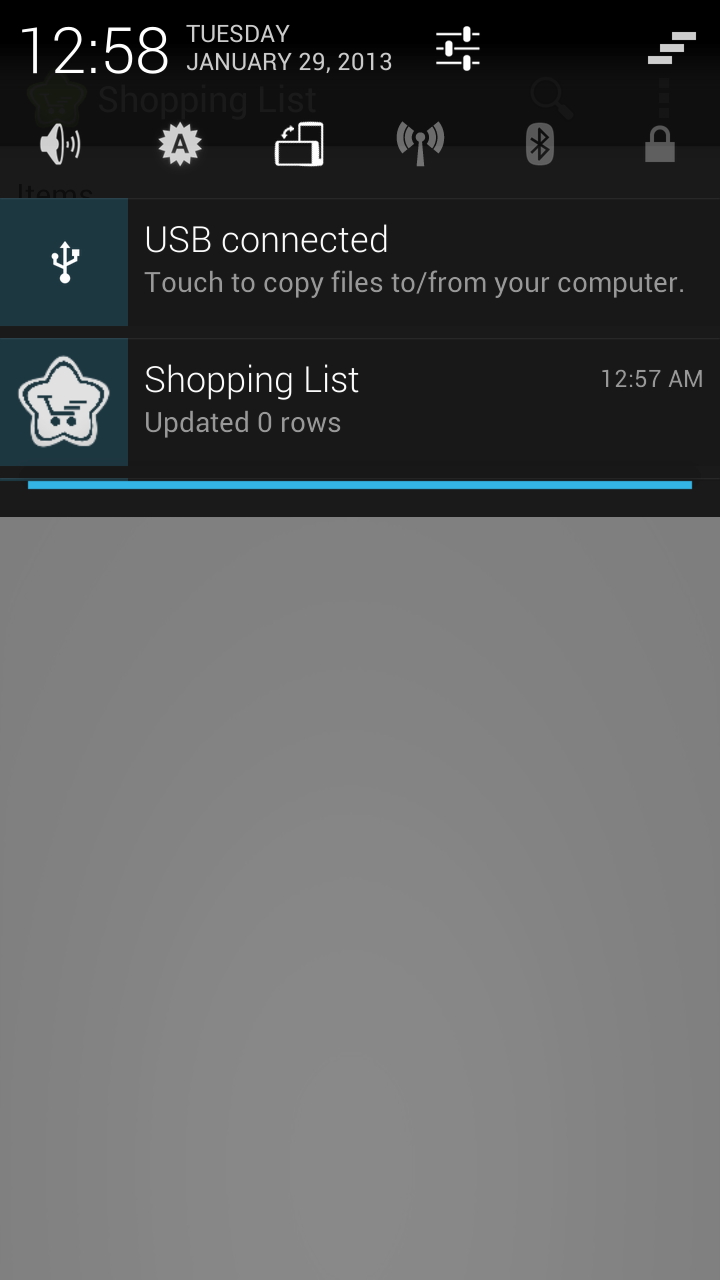
\includegraphics[width=0.25\textwidth]{images/dl.png}
\caption{ShoppingList after first sync.}
\label{fig:first_sync}
\end{figure}

This will cause the client to request the appropriate SQL file and JSON meta
model file from the server. Using this, it will create a local version of the
database and request all missing rows (which will be all rows). It will finish
by reporting the total amount of rows that it received, as seen in
Figure~\ref{fig:first_sync}


%\begin{figure}[h!]
%    \centering
%    \begin{subfigure}[b]{0.1\textwidth}
%        \centering
%        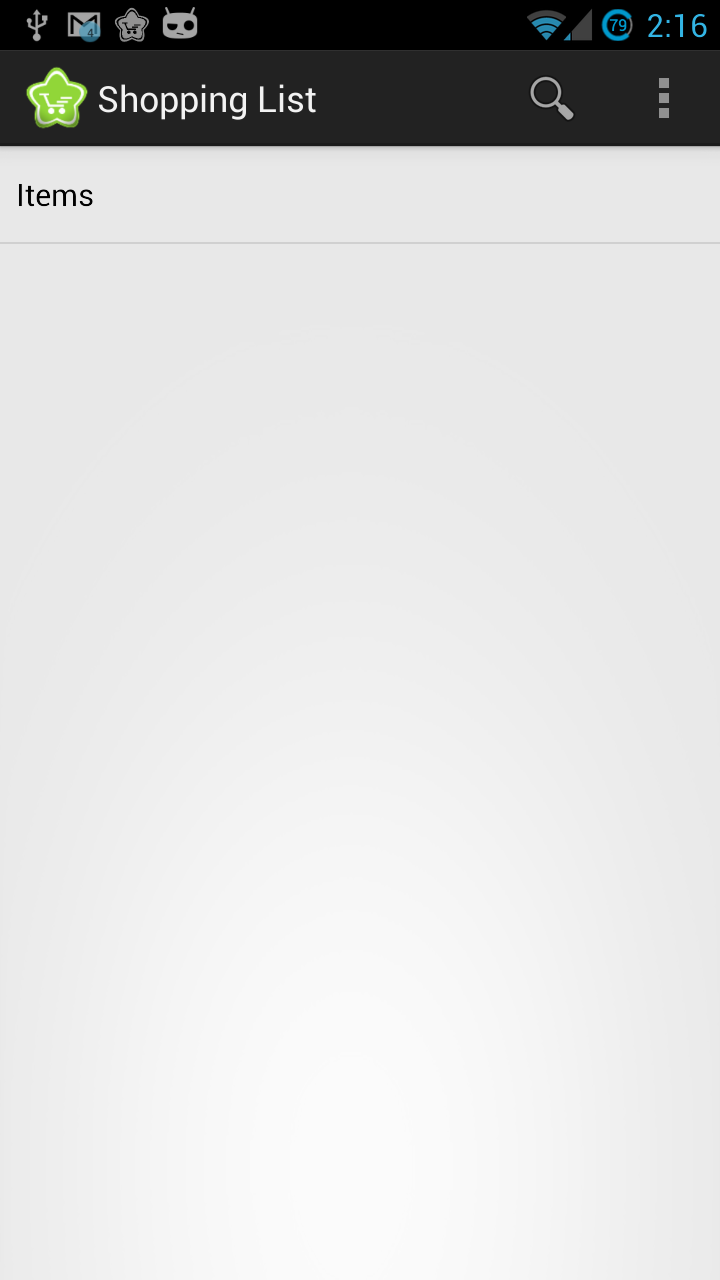
\includegraphics[width=\textwidth]{images/s1.png}
%        \caption{Home}
%        \label{fig:home}
%    \end{subfigure}%
%    ~ %add desired spacing between images, e. g. ~, \quad, \qquad etc.
%      %(or a blank line to force the subfigure onto a new line)
%    \begin{subfigure}[b]{0.1\textwidth}
%        \centering
%        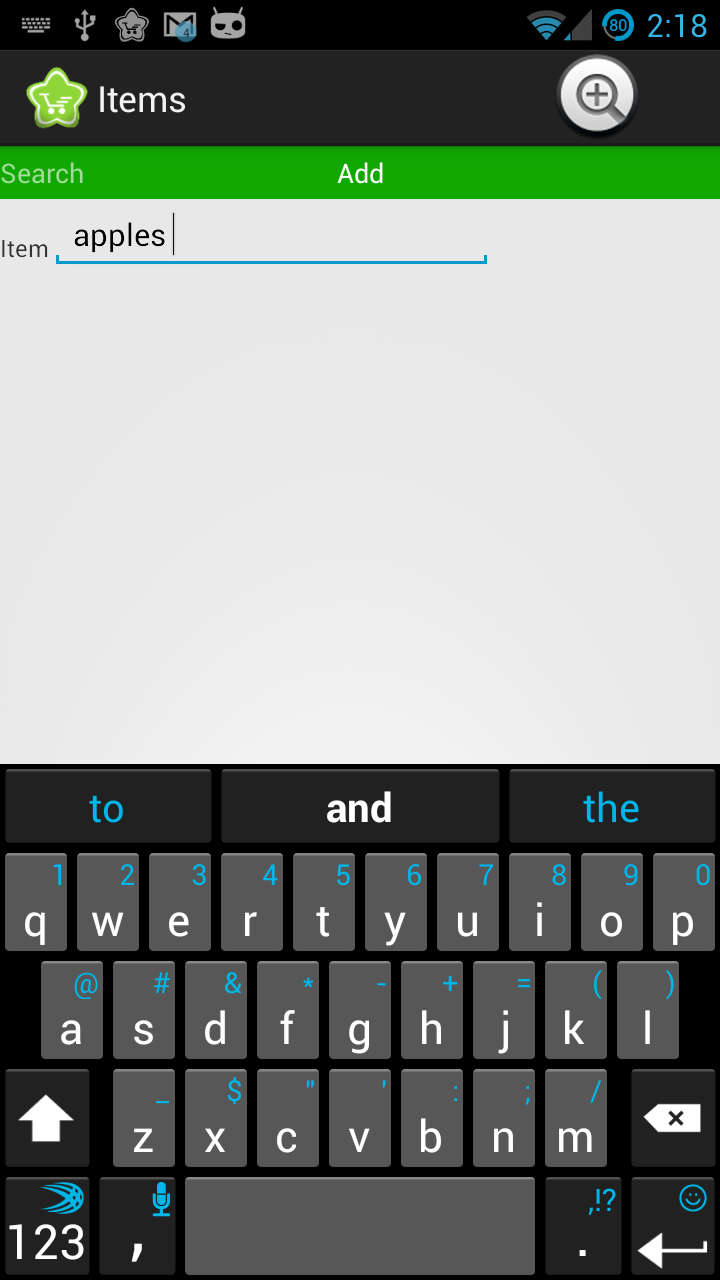
\includegraphics[width=\textwidth]{images/s2.png}
%        \caption{Add}
%        \label{fig:add}
%    \end{subfigure}
%    ~ %add desired spacing between images, e. g. ~, \quad, \qquad etc.
%      %(or a blank line to force the subfigure onto a new line)
%    \begin{subfigure}[b]{0.1\textwidth}
%        \centering
%        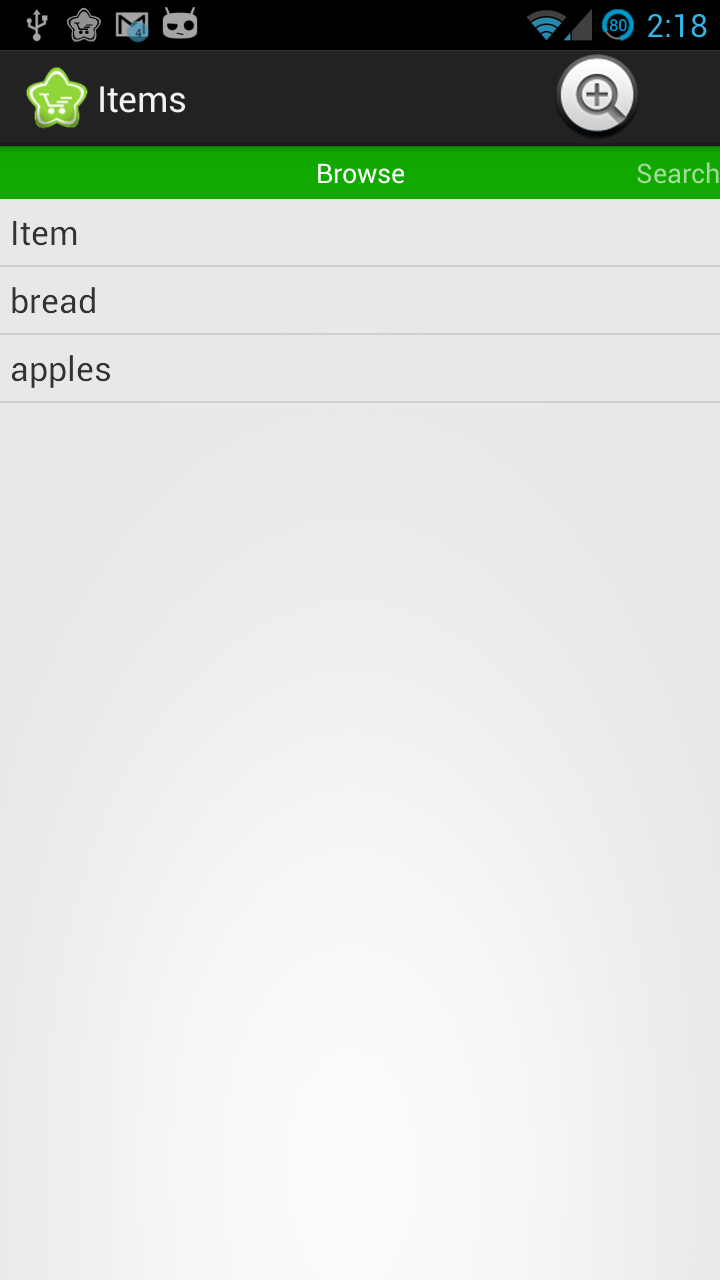
\includegraphics[width=\textwidth]{images/s3.png}
%        \caption{Browse}
%        \label{fig:browse}
%    \end{subfigure}
%    \caption{Final ShoppingList application screens.}\label{fig:shoppinglist}
%\end{figure}


At this point the application is fully functional. Clicking on the
\texttt{Items} section in the home screen will bring launch the CRUD screen for
it. Swiping to the right will reveal the UI form generated by the JSON meta
model and swiping to the left will allow browsing of the database contents. 




